\subsection*{Question 3.3}
In this question we are using this 2 equation.

\begin{equation}
	u = \frac{1}{\sqrt{\lambda_1}}k^T_1(s-\mu)
\end{equation}

\begin{equation}
	v = \frac{1}{\sqrt{\lambda_1}}k^T_1(s-\mu)
\end{equation}

Wher k_1 and k_2 is the egenvectors for the to best egenvalues. we use the orindenel data from the hans to find there diverrens from this 2 hans. and plot are scatter plot over then diferens, se figur \ref{fig:q33scatter}, wher 0 in the x and y axes, is the best posibol selution.

\begin{figure}[!htbp]
  \centering
  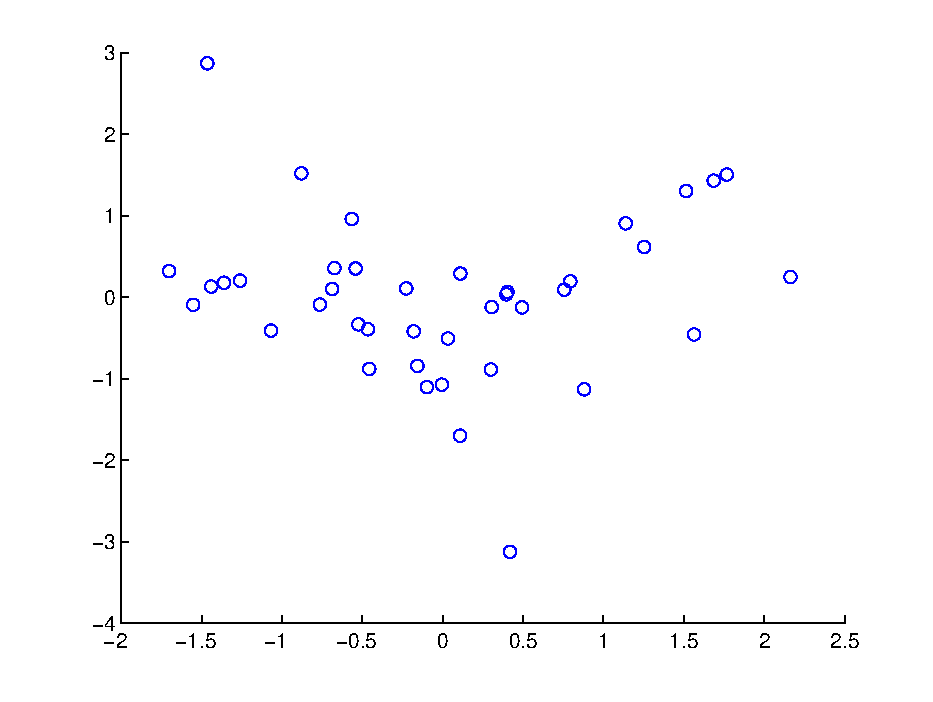
\includegraphics[width=0.85\textwidth]{./images/q33_scatter}
  \caption{Shows a scatter plot over the diffrens  plot over the first hand in the data set.}
  \label{fig:q33scatter}
\end{figure}



\begin{figure}[!htbp]
  \centering
  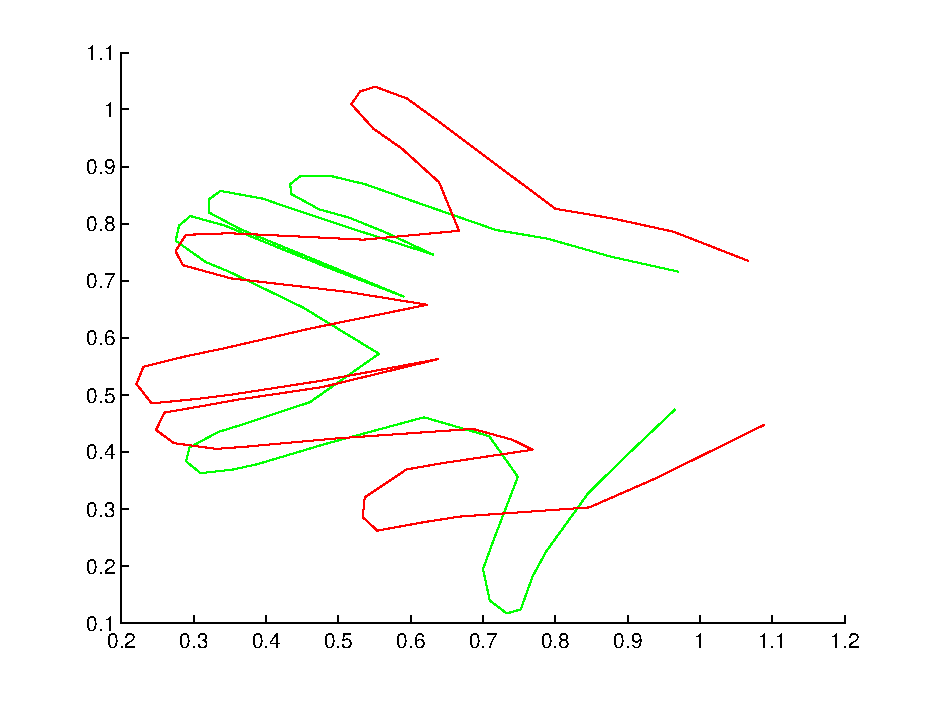
\includegraphics[width=0.85\textwidth]{./images/q33}
  \caption{To hans wher the worst fit is the green hand and the sekedt vorst is the red hand.}
  \label{fig:q33}
\end{figure}




